\chapter[Longevity]{Ecology and mode-of-life explain lifespan variation in birds and mammals}
\label{chap:Longevity}


\begin{figure}[h]
  \centering
  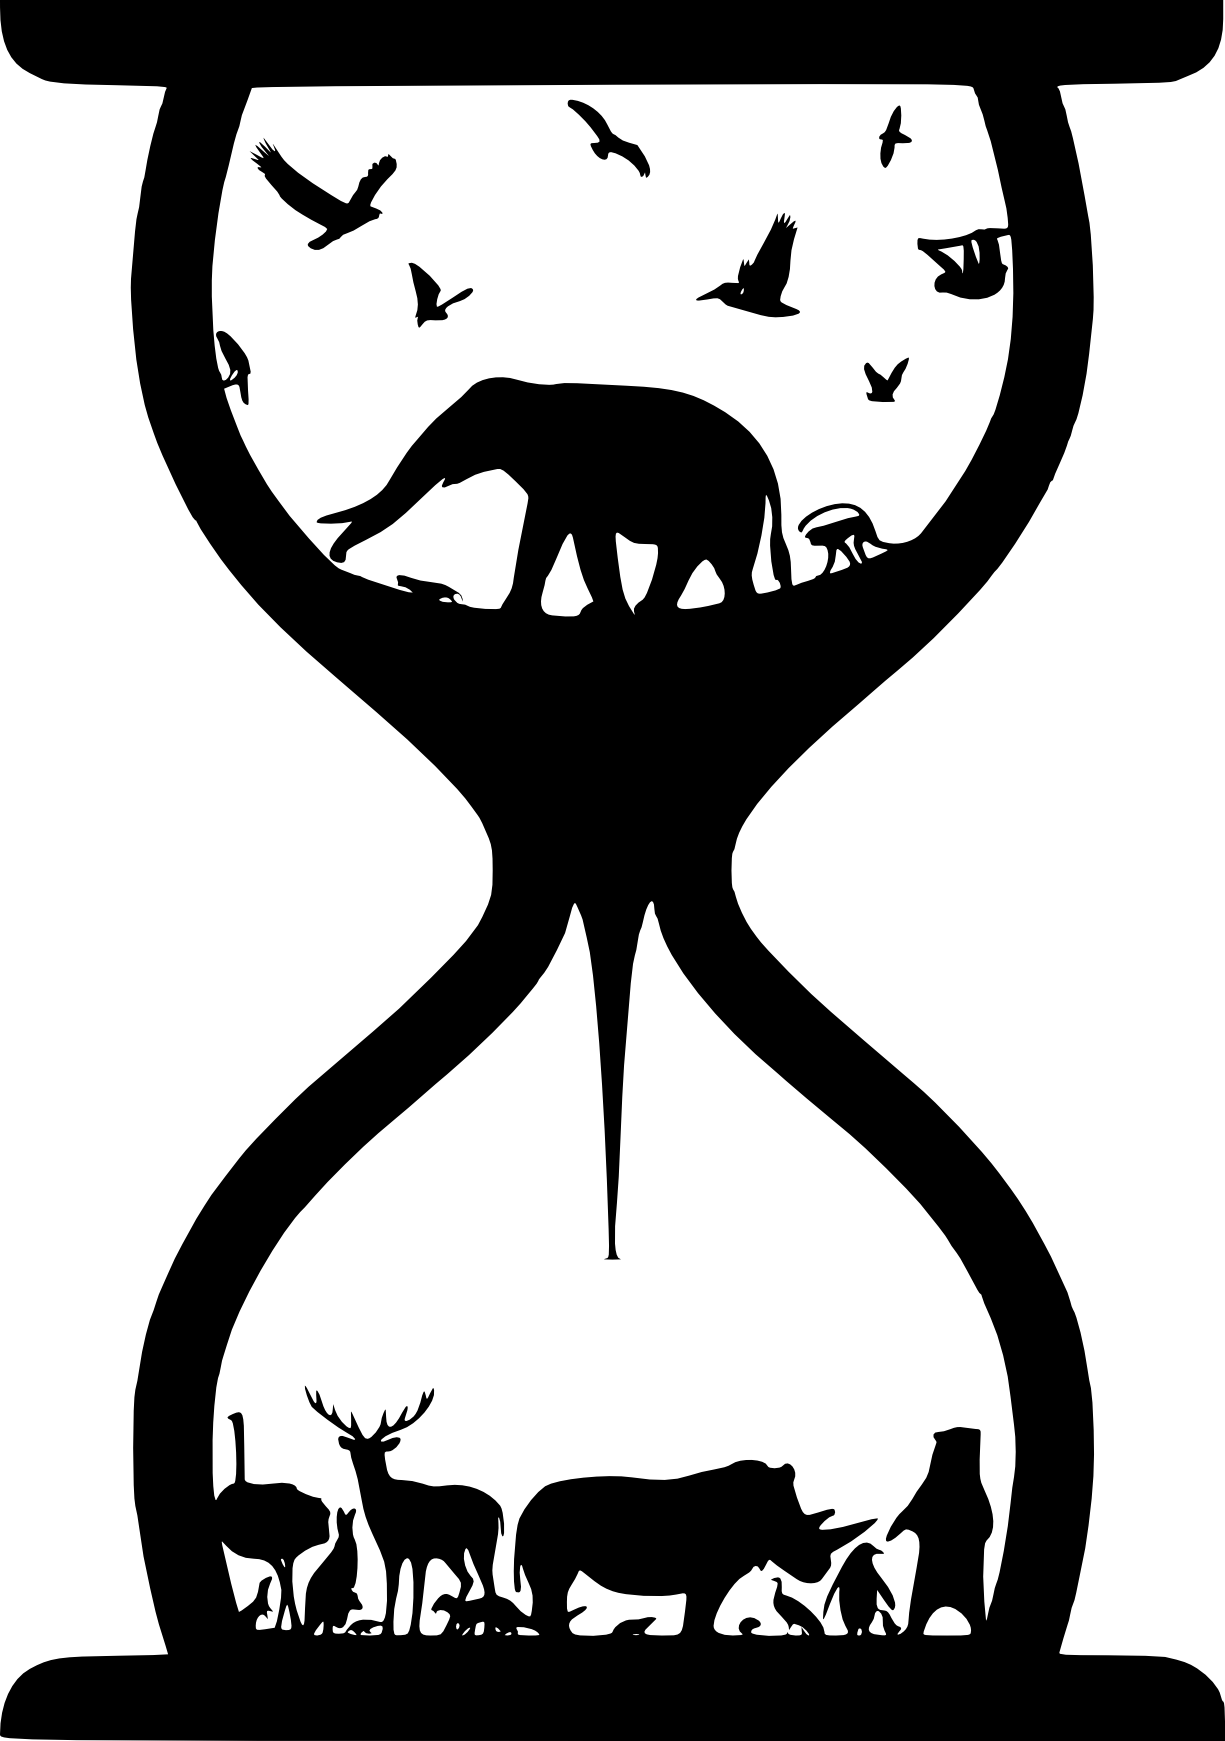
\includegraphics[width=.20\textwidth]{ch3-longevity/long.png}
\end{figure}


\begin{quoteshrink}
  ``Achieving life is not the equivalent of avoiding death.''
  
\hfill{Ayn Rand}
\end{quoteshrink}

%%%%%Always keep your smile. That's how I explain my long life. Jeanne Calment



\begin{abstract}
Many species live far longer than expected given their body mass. This may reflect interspecific variation in extrinsic mortality, with species capable of reducing mortality expected to exhibit longer lifespans. One such factor that may strongly influence such extrinsic mortality is habitat dimensionality. As higher dimensional habitats create multiple escape routes from predation, species associated with such environments would be expected to have higher maximum lifespans. Here, I investigate how such traits associated with habitat dimensionality inducing volancy, arboreality and fossoriality, along with other potential traits, including activity patterns and eusociality, influence lifespan across birds and mammals. Using phylogenetic comparative analyses with over 1300 species I show that, over and above the effect of body mass, species associated with high dimensional habitats, through arboreality and the ability to fly, live the longest. Within volant species, lifespan depended upon when (activity patterns), but not where (foraging habitats), species are active. However, the opposite was true for non-volant species, where lifespan correlated positively with both arboreality and whether they were eusocial. These results indicate that dimensionality can affect the ability of prey to escape predation with the resulting affects on species life-history evolution. 

\end{abstract}

\section{Introduction}

Lifespan, or longevity, is a fundamental life-history trait that exhibits considerable variation both within and among species. Maximum lifespan in vertebrates, for example, ranges from up to 211 years in the bowhead whale (Balaena mysticetus;\citep{de2009database}), down to just eight weeks in the pygmy goby (Eviota sigillata; \citep{depczynski2005shortest}). Like most other life-history traits, lifespan varies strongly with body size such that large species tend to live longer than smaller species \citep{lindstedt1981body,promislow1993size,de2007analysis,ricklefs2010life}. However, many species have far longer, or indeed shorter, lives than expected given their body mass (Figure 1). Understanding the mechanisms underlying these deviations from predicted lifespan may reveal the secrets to treating and combating human ageing \citep{ricklefs2010insights,zhang2013comparative}. 

One explanation for species living longer than expected, given their body size, is that low extrinsic mortality (i.e. low risk of death due to external causes such as disease, predation, food shortages  or accidents) will, on average, select for longer lifespans than when extrinsic mortality is high \citep{stearns1992evolution,Williams1957}. This is because when untimely death is more likely, investment in early and frequent reproduction is favoured rather than investment in long-term maintenance and survival. Therefore, species with adaptations that reduce the risks of extrinsic mortality should live longer than expected, given their body mass \citep{partridge1993optimality}. These ideas have led to myriad, taxon-specific hypotheses about traits that may reduce extrinsic mortality and result in increased lifespan (reviewed in \cite{ricklefs2010insights}). However, there is little consensus about the general drivers of increased lifespan across clades.

As predation is one of the main sources of extrinsic mortality, species which possess the ability to reduce it, for example through the use of toxin defences, show increased lifespans [ref]. One fundamental ecological aspect that would be expected to affect such predation pressures is the dimensionality of the habitat a species lives within. The dimensionality of trophic interactions is a key element in predation pressures where consumption rates scale higher with body mass in high dimensional interactions \citep{pawar2012dimensionality}. While this increased scaling of potential predation pressures may be expected to decrease prey species longevity in such environments the converse may also be expected through the increase ability of prey species to escape due to the increased availability of escape routes in terms of directionality and cover. Two such common ways a species may access such escape paths include arboreality and the ability to fly.

The ability to fly, and thus more easily escape predation and unfavourable conditions, is perhaps the most effective way a terrestrial species can evolve to reduce its extrinsic mortality and increase its lifespan \citep{partridge1993optimality,holmes1994fly,pomeroy1990fly}. This is supported strongly by striking differences in the lifespan of volant (flying) and non-volant (non-flying) vertebrates; on average, bats live 3.5 times longer than similarly-sized non-volant placental mammals \citep{wilkinson2002life,austad1991mammalian}, while birds live up to four times longer than similarly sized mammals \citep{lindstedt1981body,holmes2003birds}. Similarly aeboeriality has also been cited as extending longevity in species mainly through decreasing predations risks \citep{shattuck2010arboreality}. However, these may not be the only route to reducing extrinsic mortality and thereby increase lifespan. Ecological factors may also be important. Previous studies have investigated the relationship between lifespan and various ecological variables, but most only investigated select groups of species and few considered multiple traits simultaneously (e.g. \cite{shattuck2010arboreality}).

Here I investigate how multiple ecological and mode-of-life traits simultaneously influence maximum lifespan across birds and mammals. I test several hypothesis regarding the relationships among lifespan and ecological and mode-of-life traits known to influence extrinsic mortality risk; including flight capability (volant or non-volant), activity period (diurnal, crepuscular [i.e. active at dawn and dusk], nocturnal or cathemeral [i.e. active both day and night]), foraging environment (terrestrial, semi-arboreal, arboreal, aerial or aquatic), and fossoriality (i.e. living in burrows; fossorial, semi-fossorial, non-fossorial). I approach these questions by using the largest number of species to date in such an analysis (N =  589 birds and 779 mammals) and by using the most up to date phylogenetic comparative approach that includes using a distribution of 500 combined bird and mammal phylogenies to control for the phylogenetic autocorrelation introduced by shared ancestry \citep{harvey1991comparative} and body mass \citep{lindstedt1981body}.


I predict that, after controlling for body mass, species which can accesses escape routes within high dimensional habitats including (i) volant and arboreal species will either show reduced or enhanced lifespans in comparison to other species; (ii) semi-arboereal, semi-aquatic and semi-fossorial species which can seek refuge across different environments would be expected to live longer then terrestrial species; Species with nocturnal, crepuscular or cathemeral activity patterns will live longer than diurnal species, because species that are active at night or dusk are likely to be harder for predators to detect \citep{holmes1994fly,promislow1990living}; and (4) fossorial (i.e. species that live in permanent burrows) will live longer than purely terrestrial species, because they possess means to escape predation and unfavourable conditions through refuge \citep{buffenstein2002naked}.

As ecological factors that influence lifespan are likely to vary among volant and non-volant species because sources of extrinsic mortality will differ in these two groups, these groups were split species into volant (most birds and all bats), and non-volant (some birds and most mammals) subgroups, to discover general, broad-scale correlates of lifespan in endotherms, rather than separate correlates for birds and mammals. I then tested the above hypotheses on volant and non-volant species separately. As predicted, after controlling for body mass and phylogeny, volant and arboreal species live longer then terrestrial species. Surprisingly of the species capable of transitioning across environments only semi-arboreal species showed increased lifespan while only volant crespucular species showed any effect of activity period on longevity.

\section{Materials and Methods}
\subsection{Data}

We used maximum longevity as our measure of lifespan as it is thought to be the best available estimator of a species' ageing rate \citep{de2007analysis} and because of the amount of high quality longevity data available. We obtained data on maximum longevity (years) and adult body mass (g) from the AnAge database \citep{de2009database,tacutu2012human}. In our main analysis we excluded species with maximum longevity estimates based on fewer than ten longevity records, or with low or questionable data quality as defined in the AnAge database \citep{de2007analysis}. As maximum values are dependent on sample size we also ran a sensitivity analysis excluding species with maximum longevity estimated from fewer than 100 longevity records. Note that longevity records for non-volant mammals tend to come from captive individuals, whereas data for bats and birds tend to come from wild caught individuals. Although we expect captive individuals to live longer than wild individuals, on average maximum longevity tends to remain unchanged between captive and wild populations \cite{ricklefs2001comparison}. Further, given that bats and birds live longer than non-volant mammals, this should make our analyses more conservative. 

To test our hypotheses concerning the relationships between lifespan, mode-of-life and ecological traits, we collected data on the flight capability (volant or non-volant), activity period (diurnal, crepuscular, nocturnal or cathemeral), foraging environment (terrestrial, semi-arboreal, arboreal, aerial or aquatic), and fossoriality (fossorial, semi-fossorial or non-fossorial) of each species using Walker's Mammals of the World \citep{nowak1999walker}, the Handbook of Birds of the World series \citep{hoyo1992handbook}[25], the Handbook of the Birds of Europe, the Middle East and North Africa series \citep{cramp1977handbook} and some additional sources (Appendix 1, \citep{fry2010kingfishers,parr2010parrots,williams1995penguins}). These categories are described in detail in Appendix 1. We used the taxonomy of Wilson and Reeder \citep{wilson2005mammal} for mammals and Jetz et al. \cite{jetz2012global} for birds. We excluded purely aquatic mammals (Cetacea and Sirenia) from the analyses because we expect selection pressures to be very different in these groups. We also excluded gliding mammals because there were too few species (N = 9) to run a separate analysis and because this group could equally fit into either the volant or non-volant subgroups.

Rather than basing our analyses on just a single phylogenetic tree and assuming this tree was known without error, we instead used a distribution of trees. We extracted 500 bird trees from the posterior distribution of a recent bird phylogeny generated under a Bayesian inference framework \citep{jetz2012global}, and used the 10,000 mammal trees constructed by Kuhn et al. \citep{kuhn2011simple}. Each individual mammal tree comprises one resolution of the polytomies of a previously published supertree \citep{bininda2007delayed}. We treat these as equivalent to a Bayesian posterior distribution of trees because no such tree analysis exists for all mammals. As we needed a distribution of phylogenies containing both birds and mammals, we randomly selected one bird tree and one mammal tree (without replacement) and bound them to make a combined tree. The trees were bound with a root age of 315 million years, corresponding to the fossil calibration for all amniotes, i.e.,  \textit{Archerpeton anthracos} (Appendix 1; \citep{reisz2004molecular}). We repeated this procedure 500 times to generate a distribution of 500 combined bird and mammal trees.

Many studies on vertebrate ageing have noted a strong correlation between maximum longevity and metabolic rate. Opinion is divided as to whether this is a causative relationship or merely confounded with the strong correlation between body mass and metabolic rate \citep{ricklefs2010insights}. To determine whether our conclusions hold when we include metabolic rate in our models, we also compiled mass-specific basal metabolic rate (BMR; Wg-1) data (see Appendix 1).


In total our analyses used data from 589 birds (579 volant and 10 non-volant) and 779 mammals (83 volant and 696 non-volant; see Appendix 3: Table A1 for more details and Appendix 2 for the complete dataset). This was reduced to 112 birds and 330 mammals when we include BMR in our models, and 474 birds and 435 mammals in the sensitivity analysis using only species with 100 or more longevity records.

\subsection{Analyses}

To test our hypotheses we fitted the following three models, with Maximum longevity and Body mass incorporated as continuous variables; Flight capability, Foraging environment, Activity period and Fossoriality as factors and with Body mass:Flight capability representing the interaction between Body mass and Flight capability:


\begin{enumerate}
  \item For all species (N =1368:
Maximum longevity = f(Body mass +  Flight capability + Body mass: Flight capability)
  \item For volant species only (N = 662):
Maximum longevity = f(Body mass + Foraging environment + Activity period)
  \item For non-volant species only (N =706):
Maximum longevity = f(Body mass +  Foraging environment + Fossoriality + Activity period)
\end{enumerate}


All analyses were carried out in R v3.0.2 \citep{RCran}. Maximum longevity and body mass (and BMR, see below) were log10 transformed to correct inherent skewness before being mean centred and expressed in units of standard deviation.
We fitted our models using Bayesian phylogenetic mixed models from the MCMCglmm package \citep{hadfield2010mcmc}, to account for non-independence in species traits introduced as a result of common ancestry \citep{harvey1991comparative}. MCMCglmm uses a Markov chain Monte Carlo estimation approach and accounts for non-independence among closely-related species by including the phylogenetic relationships among species as a random variable. We determined the number of iterations, thinning and the burn-in period for each model run across all trees using diagnostics in the coda package \citep{plummer2006coda} and we checked for convergence between model chains using the Gelman-Rubin statistic, the potential scale reduction factor (PSR), with all models required have a PSR below  1.1 \citep{gelman1992inference}. Following the recommendations of Hadfield \citep{hadfield2010mcmc}, we used an uninformative inverse-Wishart distribution (with variance, V, set to 0.5 and belief parameter, nu, set to 0.002) and a parameter expanded prior, with a half-Cauchy distribution (described by the parameters V = 0.5, nu = 1, the prior mean alpha.mu = 0, and alpha.V = 102, which represents the prior standard deviation with a scale of 10), for the random factor to improve mixing and decrease autocorrelation among iterations. 

As noted above, rather than using one phylogenetic tree and assuming this tree was error free, we instead used a distribution of 500 combined bird and mammal trees and fitted each of our models to each of these trees. We then combined the resulting model outputs to give model estimates which incorporate the error across the 500 trees.  As the posterior outputs of MCMC models are combinable, coefficient distributions were created by amalgamating each coefficient posterior. 

To determine whether our conclusions held when we excluded species with fewer than 100 longevity records or when metabolic rate was included in our models, we repeated models 1-3 with either the reduced dataset of species with 100 or more longevity records or with BMR as an additional linear covariate. We also repeated Models 2 and 3 for birds and mammals (rather than volant and non-volant species) separately to ensure that differences between the volant and non-volant subgroups were due to differences in flight capability and were not simply representing the difference between mammals and birds. We calculated the deviance information criteria (DIC), a hierarchal generalization of AIC, for each bird and mammal paired models and compared it to the paired volant and non-volant models to compare model "fit" of each approach.

Finally, Since publication of this work \citep{healy2014ecology} new analysis performed by \cite{williams2015ecology} outlined the potential importance of eusociality in small mammals associated with fossoriality. The analysis uses the data described above along with new data on eusociality, defined using reproductive skew \citep{williams2015ecology}, to show that eusociality is also a predictor of increased maximum lifespans. To further analysis this composite dataset I used the methods outlined above to investigate the importance of eusociality while controlling for phylogeny and the error within phylogenetic reconstructions.

\section{Results}

The analysis show that volant species live longer than non-volant species of a similar body mass (Table 1, Figure 1). In addition, for a given increase in body mass, the lifespans of volant species (modal slope estimate [after converting from mean-centred values] = 0.25; Table 1) increase significantly more than the lifespans of non-volant species (modal slope estimate [after converting from mean-centred values] = 0.13; Table 1).


\begin{table}[h]
  \caption[Table 1.]{Relationship between maximum longevity (years), body mass (g) and flight capability (volant or non-volant) in 1368 birds and mammals. Estimates are modal estimates from 500 models. Lower CI = Lower 95\% confidence interval from 500 models. Upper CI = Upper 95\% confidence interval from 500 models. Posterior distribution = distribution of estimates from 500 models. Body mass \: Flight capability = interaction between body mass and flight capability.}
  \label{tbl:Table 1.}
  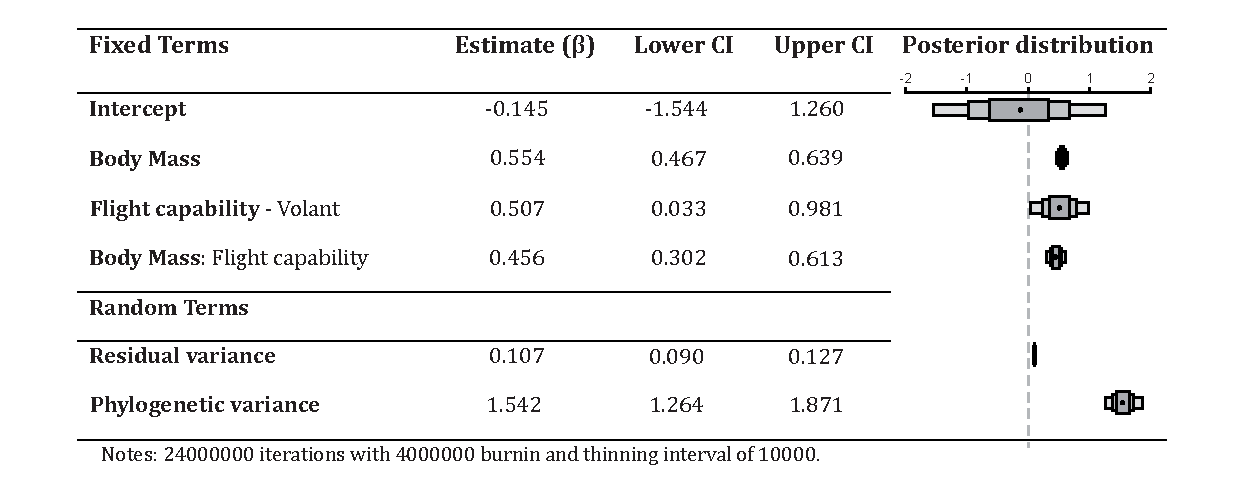
\includegraphics[width=\linewidth]{ch3-longevity/Table1.pdf}
\end{table}


\begin{figure}[p!]
  \centering
  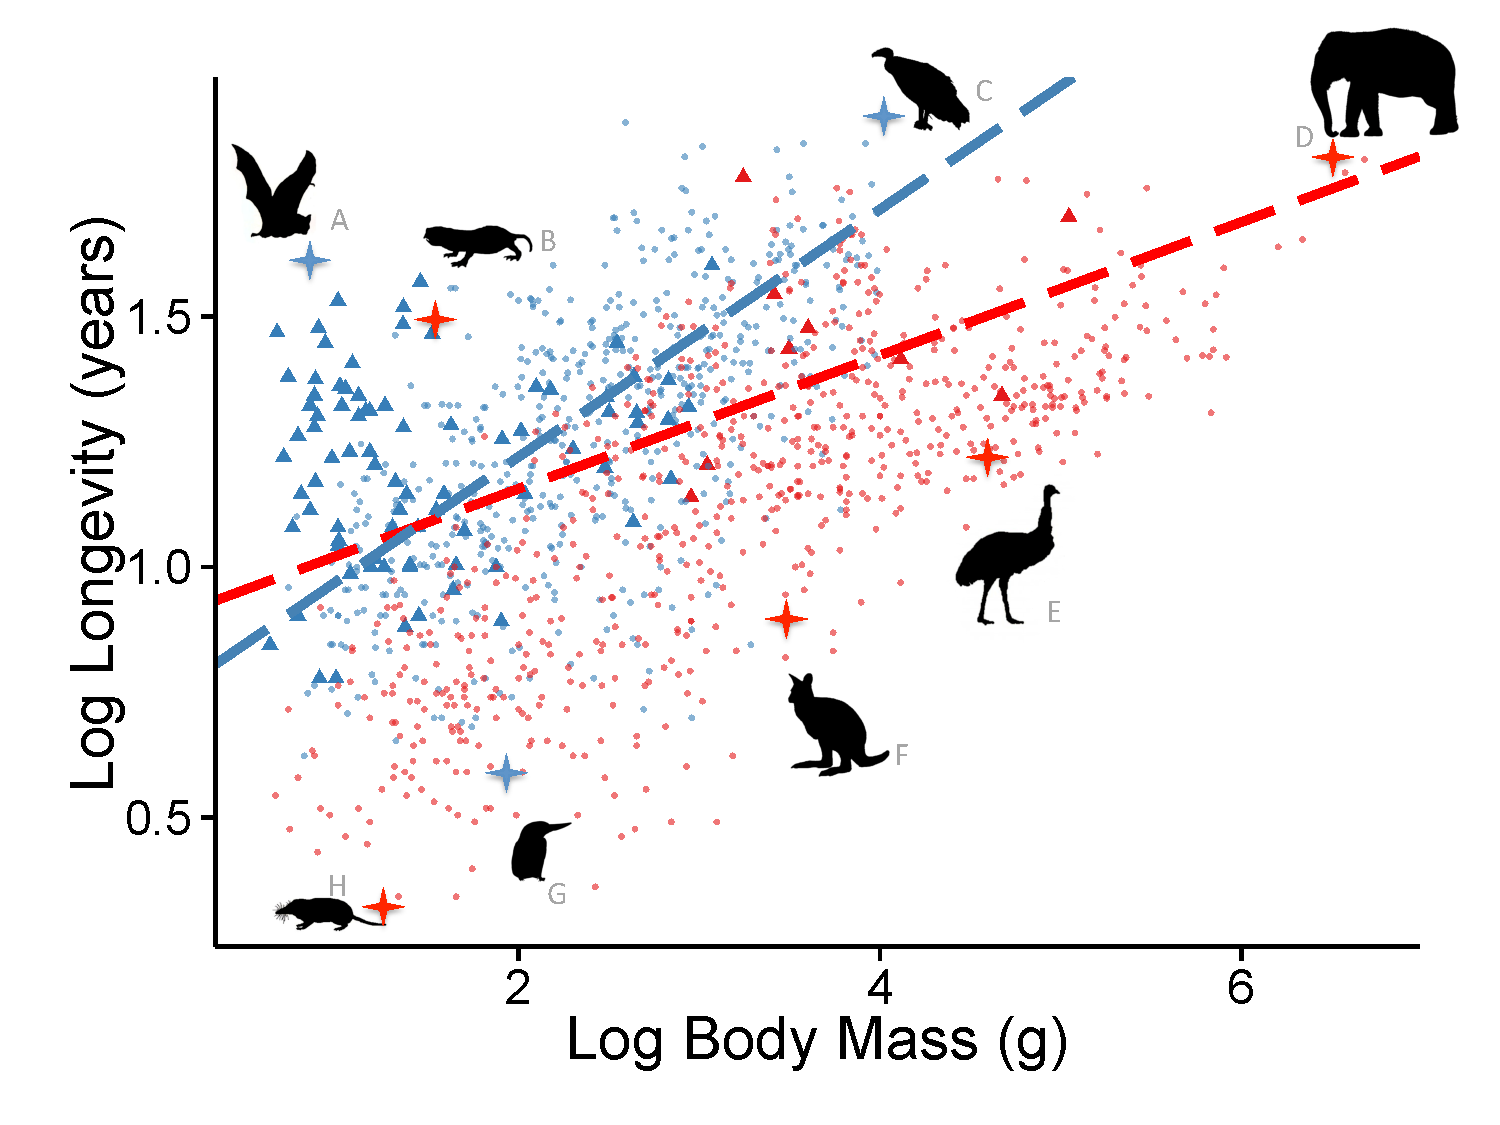
\includegraphics[width=1.0\textwidth]{ch3-longevity/Figure1.pdf}
  \caption[Figure 1.]{Relationships between body mass and maximum lifespan in birds and mammals. Silhouettes highlight a selection of species with much longer or shorter lifespans than expected given their body size. These species are (A) \textit{Myotis brandtii}, Brandt's bat; (B) \textit{Heterocephalus glaber}, Naked mole rat; (C) \textit{Vultur gryphus}, Andean condor; (D) \textit{Loxodonta Africana}, African elephant; (E) \textit{Dromaius novaehollandiae}, Emu; (F) \textit{Dorcopsulus macleayi}, Papuan forest-wallaby; (G) \textit{Ceryle rudis}, Pied kingfisher; and (H) \textit{Myosorex varius}, Forest shrew. Blue points and line represent volant birds and mammals (N = 662; slope = 0.25, intercept = 0.73). Red points and line represent non-volant birds and mammals (N = 706; slope = 0.13, intercept = 0.89). Blue triangles represent bat species and red triangles represent non-volant bird species. Estimates of slopes and intercepts represent back transformed values from mean centred values given in Table 1.}
  \label{figure:Figure 1.}
\end{figure}


The relationships among our ecological variables and lifespan differed between the volant and non-volant subgroups. Within volant taxa, crepuscular species (i.e. those active at dusk and dawn) had significantly shorter lifespans than both diurnal and nocturnal species (Table 2). In contrast, activity period was not associated with lifespan in non-volant species (Table 3). Foraging environment did not influence lifespan significantly in volant species; bats and birds that forage on the ground do not have shorter lifespans than species that forage in the air or in trees (Table 2). Within non-volant species, however, those foraging arboreally have longer lifespans than those foraging terrestrially, and fossorial (i.e. burrowing) species live longer than non-fossorial ones (Table 3).


\begin{table}[h]
  \caption[Table 2.]{Relationship between maximum longevity (years), body mass (g), foraging environment and activity period in 662 volant birds and mammals. Estimates are modal estimates from 500 models. Lower CI = Lower 95\% confidence interval from 500 models. Upper CI = Upper 95\% confidence interval from 500 models. Posterior distribution = distribution of estimates from 500 models.}
  \label{tbl:Table 2.}
  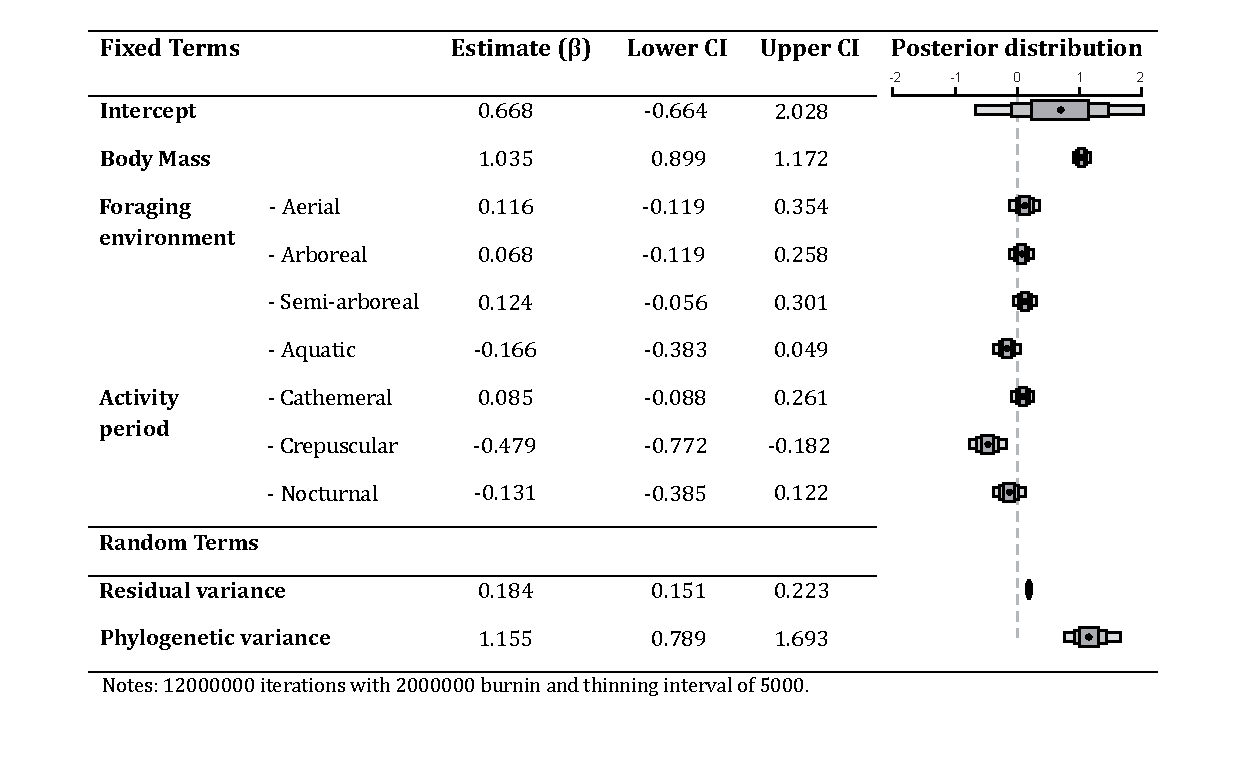
\includegraphics[width=\linewidth]{ch3-longevity/Table2.pdf}
\end{table}


\begin{table}[h]
  \caption[Table 3.]{Relationship between maximum longevity (years), body mass (g), foraging environment, fossoriality and activity period in 706 non-volant birds and mammals. Estimates are modal estimates from 500 models. Lower CI = Lower 95\% confidence interval from 500 models. Upper CI = Upper 95\% confidence interval from 500 models. Posterior distribution = distribution of estimates from 500 models.}
  \label{tbl:Table 3.}
  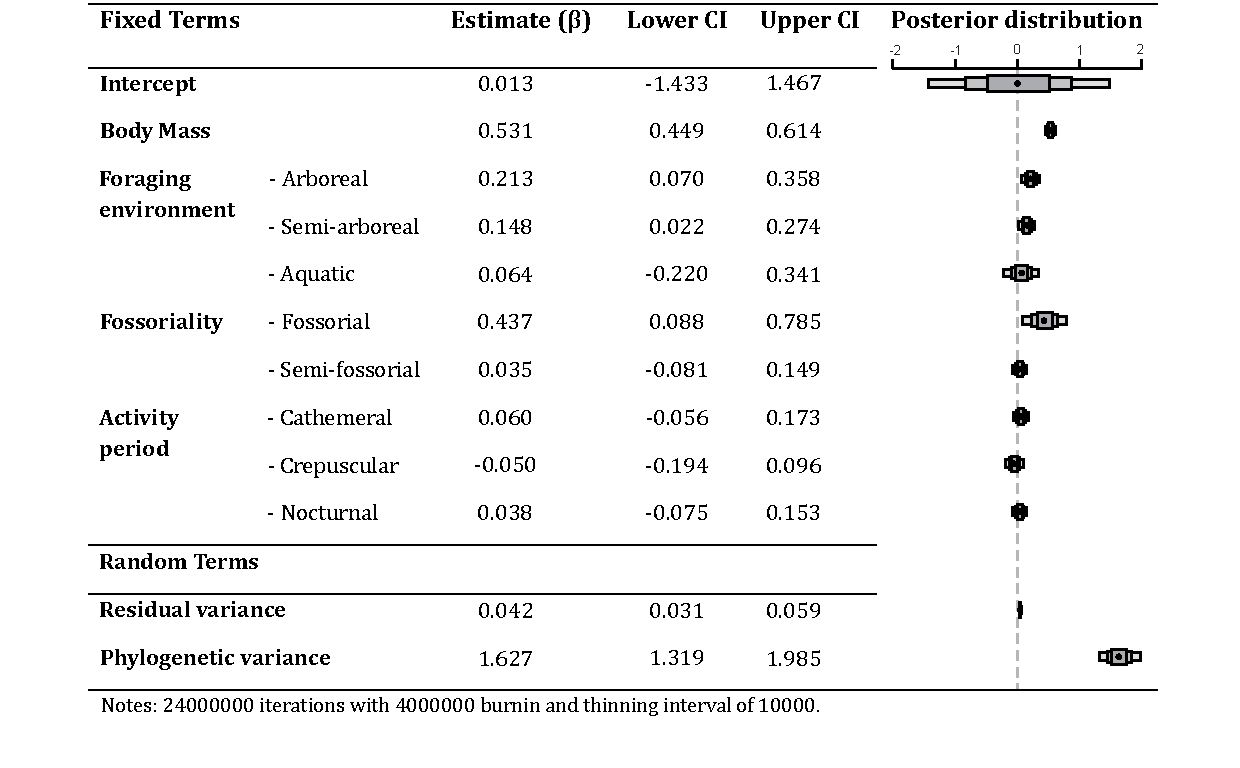
\includegraphics[width=\linewidth]{ch3-longevity/Table3.pdf}
\end{table}


\begin{table}[h!]
  \caption[Table 4.]{Relationship between maximum longevity (months), body mass (g), sociality (eusocial or no-eusocial) and fossoriality (fossorial non-fossorial). Estimates are modal estimates from 25 models. Lower CI = Lower 95\% confidence interval from 25 models. Upper CI = Upper 95\% confidence interval from 25 models. Posterior distribution = distribution of estimates from 25 models.}
  \label{tbl:Table 4.}
  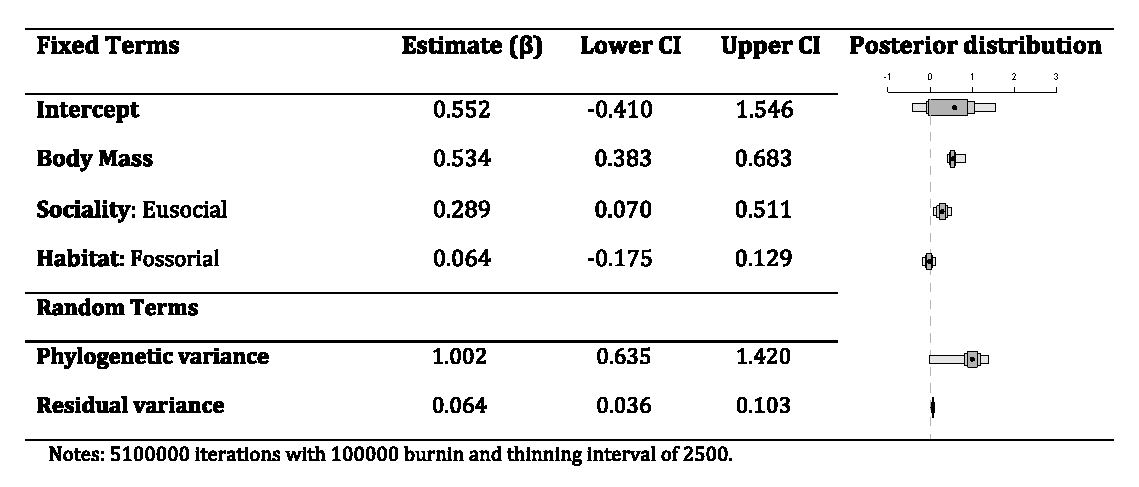
\includegraphics[width=\linewidth]{ch3-longevity/Table4.pdf}
\end{table}



In the supplementary analysis with maximum longevity estimates based on 100 or more records, the models showed qualitatively comparable results to the findings in the main analysis (Appendix 3: Tables A2-A4). When we included BMR as an additional linear covariate into Models 1-3, the results showed similar general trends as those without BMR except with no significant effect of crepuscularity in volant species, no effect of semi-arboreality in non-volant species and a negative correlation between BMR and longevity in non-volant species (Appendix 3: Tables A5-A7).  We also repeated Models 2 and 3 for birds and mammals (rather than volant and non-volant species) separately. The results were qualitatively identical apart from a predictable reduction in the phylogenetic residual term and also a lower combined DIC value for Models 2 and 3 (modal volant and non-volant DIC = 1184) in comparison to a taxonomically split model (modal birds and mammals DIC  = 1227) (Appendix 3: Tables A8-A9). The phylogenetic residual term was high in all of our models (model 1: 1.542; model 2: 1.555; model 3: 1.627; Tables 1-3) but was much lower in the taxonomically split bird and mammal models, as expected given their more restricted phylogenetic scope (birds: 0.371; mammals: 0.936; Appendix 3, Table A10). Finally, the additional analysis of \cite{williams2015ecology} dataset showed that eusociality but not fossoriality (as defined to include both semi-fossorial and fully fossorial species; Table 4).



\section{Discussion}

As predicted, we found that species capable of exploiting high dimensional environments live longer than species of a similar body mass in environments of lower dimensionality. Volant species, in particular those with nocturnal, cathemeral and diurnal activity patterns, lived longer then non-volant species while the longest-lived non-volant species tended to be arboreal or semi-arboreal. The link between these traits and increased lifespan are in line with previous studies on lifespan evolution in endotherms. Among birds, flightless or weakly-flying species (i.e. game birds) have the shortest lifespans \citep{ricklefs2010life,Williams1957,wilkinson2002life} while among mammals, bats live far longer than similarly sized non-volant mammals (ref). Arboreality is also strongly associated with longer lifespans \citep{shattuck2010arboreality} while gliding species, which mix elements of both arboeriality and volancy, also have greater lifespans than expected given their body mass \citep{holmes1994fly}. This increased lifespan is likely associated with the decreased predation pressures associated with living within high dimensional environments.


High dimensional environments may reduce predation risks through providing refuge that predators cannot access and through providing more escape routes in terms of directionality. Prey escape strategies often involve retreating to a refuge that cannot be accessed by the predator in pursuit, such as transiting between terrestrial, arboereal, aquatic or fossorial environments. However these results suggest that this is not a major contributor to lifespan evolution as semi-aquatic and semi-fossorial species show no difference in longevity in comparison to fully terrestrial species. The increased longevity in higher dimensional environments may hence better reflect the increased options available for escape in such habitats. In fact birds species that escape along vertical flight trajectory's (3D) have been found to have longer lifespans in comparison to those that use horizontal escape routes \citep{moller2010up}. 


Another explanation for the disparity between the expected decrease in longevity with due to increased predation rates with body size in high dimensional habitats \citep{pawar2012dimensionality} and these findings is that the environments included within this analysis restrict large predators. Unlike marine environments aerial and arboreal environments several restricts body size through biomechanical constraints. This is seen in the largest known aerial predators, \textit{Argentavis}, reaching only 70 kg \citep{chatterjee2007aerodynamics} while the largest extant terrestrial predators reaching up to 1000 kg \citep{carwardine1995guinness}, with extinct theropods species reaching over 15 tonnes \citep{therrien2007my}. Similarly arboreal predators are restricted by the weight branches can support with the largest such predators, felids, generally restricted to ticker branches. This exclusion of large body size species may also explain the difference in how lifespan scaled with body mass found in volant and non-volant species. While previous studies generated similar slopes for the relationship between log lifespan and log body mass in birds (slope = 0.20) and mammals (slope = 0.22) \citep{lindstedt1981body,hulbert2007life} these analysis show for a given increase in body mass, the lifespans of volant species (modal slope estimate [after converting from mean-centred values] = 0.25) increase significantly more than the lifespans of non-volant species (modal slope estimate [after converting from mean-centred values] = 0.13). This difference in scaling may reflect the relativity predator free existence of large flying species such as found in vultures and albatross.


While habitat dimensionality shows an important effect on longevity, activity patterns in both volant and non-volant species seems to show little association with lifespan. Only crepuscularity in volant species showed an effect with these species having shorter maximum lifespans. This may be a result of crespucuar species being exposed to both diurnal and nocturnal predators resulting in higher extrinsic mortality. For example bat species which emerge earliest are sucesptible to the highest predation levels \citep{jones1994foraging}. The scarcity of crepuscular volant species (N = 16) in our dataset also suggests that specialisation to be active between nocturnal and diurnal periods is a relatively unsuccessful strategy. However, activity period was not related to lifespan in non-volant species, counter to the initial prediction that nocturnal, crepuscular and cathemeral species would be more long-lived, which assumed that diurnal species would be easier for predators to detect. some link. However, there are many additional ways to avoid predation (see below) and many alternative reasons for becoming nocturnal, crepuscular or cathemeral. For example, many large mammals are crepuscular or cathemeral in order to avoid the intense heat of the day in tropical areas, while species such as wolves and hyenas may have become nocturnal to access more prey. Consequently, although nocturnality may decrease extrinsic mortality for some species, it may actually increase it for others.


Within the main analysis fully fossorial species lived longer then similar sized terrestrial species, as expected based on the inferred protection such a lifestyle may provide against predators. However subsequent analysis following \cite{williams2015ecology} showed that this association is more likley to be driven by the levels of eusociality found in fossorial species. Eusociality is also known to increase longevity through the reduce extrinsic mortality in breeding indaviduals. For example eusocial insects, perhaps the most extreme example of such a eusocial system, show a 100-fold increase in lifespan in the colony queens \citep{keller1997extraordinary}. Of the 10 fully fossorial species included in our original analysis the three species which can be best described as eusocial, the naked mole rates \textit{Heterocephalus glaber}; \textit{Cryptomys damarensism}; \textit{Spalax ehrenbergi} have maximum lifespans ranging between 15.5 and 32 years in comparison to the range of 2.5-17 years in the remaining fossorial species. This new analysis suggest that fossoriality itself does not confer additional protection from external mortality. This may be due fossoriality restricting the means of escape once encountered by a predator within the borrow. This result supports the conclusion that dimensionality is a main feature in reducing mortality in the species and may offer a  partial explanation for the exceptional longevity of naked mole rats (Heterocephalus glaber) which live ten times longer than expected, given their body size \citep{buffenstein2002naked}.



 Also following from Peto’s paradox, that cancer incidence does not correlate with body size despite the larger number of cells from which it can potentially develop [40], the increased lifespan afforded through decreased extrinsic mortality in large species can increase selection for molecular controls on senescence related diseases [11]. 


These findings highlight the potential importance of habitat complexity in lifespan evolution. The additional options for escape in such habitats may be a defining feature of throphic interactions within birds and mammals. However the biomechanical limitations associated with volancy and arboerialty, restrict the ability to draw out whether this is the causal factor behind such increased lifespans. Further comparative analysis in marine systems were such body size limitations are less restrictive and were pelagic systems are relatively clear of refuges would provide a further test to the above conclusions. In particular if habitat dimensionality is an important factor in lifespan evolution it would be expected that pelagic species live longer then similar sizes benthic species while accounting for phylogeny. Similarly other groups may help further decouple the effects of fossoriality on life history evolution. In particular comparing the diverse ecologies within reptiles would further test the effects of arboeality and fossoriality on lifespan.

Finally, while the ability to escape some of the main sources of mortality is likely to extend species lifespan and the associations between longevity and volancy, arboerality and eusocialty is clear the direct causal link is still not clear. Theoretical modelling suggests that how mortality is distributed across a species demography is a key determinant in whether that species increases its lifespan. For example reduced extrinsic mortality, especially due to predation, may increase intraspacific competition resulting in what seems as a counter-intuitive reduction in lifespan (current biology paper). To decouple such effects more detailed analysis including mortality rates across species life-histories along with comparative methods which include ecology are needed. By understanding the underpinnings of the evolution of life-history we not only provide an insight into the ecology and evolution of predator-prey interactions provide an important basis on which to view our own and understand our own ageing and  the potential to circumvent it.




\bibliographystyle{PLoS-Biology}
\bibliography{bibfile}



